\chapter{泛化}

本章将讨论理解和分析机器学习模型泛化能力的工具,即这些模型在未见过的测试样本上的表现。回想一下,对于监督学习问题,给定训练数据集 $\{(x^{(i)}, y^{(i)})\}_{i=1}^n$,通常通过最小化损失/成本函数 $J(\theta)$ 来学习模型 $h_\theta$,这鼓励 $h_\theta$ 拟合数据。例如,当损失函数是最小二乘损失(也称为均方误差)时,有 \(J(\theta) = \frac{1}{n} \sum_{i=1}^n \left(y^{(i)} - h_\theta(x^{(i)})\right)^2\) 这个用于训练的损失函数通常被称为\textbf{训练 (training)} 损失/误差/代价。

然而,最小化训练损失\textbf{并非}最终目标,它只是实现学习预测模型这一目标的途径。模型最重要的评估指标是在未见过的测试样本上的损失,通常被称为测试误差。形式上,从所谓的测试分布 $\mathcal{D}$ 中抽取一个测试样本 $(x, y)$,并衡量模型在其上的误差,例如均方误差 $(h_\theta(x) - y)^2$。测试样本随机性下的期望损失/误差称为测试损失/误差。\footnote{在理论和统计文献中,通常将训练集 $\{(x^{(i)}, y^{(i)})\}_{i=1}^n$ 上的均匀分布称为经验分布,记为 $\mathcal{D}$,将总体分布称为 $\mathcal{D}$。因此(这是一部分原因),训练损失也称为经验损失/风险/误差,测试损失也称为总体损失/风险/误差。}
\begin{equation}
    L(\theta) = \mathbb{E}_{(x,y) \sim \mathcal{D}}[(y - h_\theta(x))^2] \label{eq:8.1}
\end{equation}
请注意,误差的测量涉及计算期望,在实践中,可以通过对许多抽取的测试样本计算平均误差来近似,这些样本被称为测试数据集。这里训练集和测试集之间的关键区别在于测试样本是\textit{未见过的 (unseen)},因为训练过程没有使用这些测试样本。在经典的统计学习设置中,训练样本和测试样本都从与测试分布 $\mathcal{D}$ 相同的分布中抽取,但测试样本对于学习过程来说仍然是未见过的,而训练样本是已见过的。\footnote{近年来,研究人员越来越关注“域偏移”的情况,即训练分布和测试分布不同。}

由于训练集和测试集之间的这种关键区别,即使它们都从相同的分布 $\mathcal{D}$ 中抽取,测试误差也不一定总是接近训练误差。\footnote{训练误差和测试误差之间的差异通常称为泛化差距。泛化误差在一些文献中指测试误差,在其他一些文献中指泛化差距。} 因此,成功最小化训练误差可能并不总是导致测试误差很小。如果模型在训练集上准确预测数据,但在其他测试样本上泛化能力不好,通常说模型\textbf{过拟合 (overfits)} 数据,即训练误差小而测试误差大。如果训练误差相对较大\footnote{例如,大于回归问题中数据的内在噪声水平。}(在这种情况下,测试误差通常也相对较大),则说模型\textbf{欠拟合 (underfits)} 数据。

本章研究学习过程如何影响测试误差,特别是模型参数化的选择。将测试误差分解为“偏差”和“方差”项,并研究模型参数化的选择及其权衡如何影响它们。利用偏差-方差权衡,将讨论何时发生过拟合和欠拟合以及如何避免。还将讨论 \ref{sec:8.2} 节中的双下降现象和 \ref{sec:8.3} 节中的一些经典理论结果。


\section{偏差-方差均衡}\label{sec:8.1}

\begin{figure}[H]
    \centering
    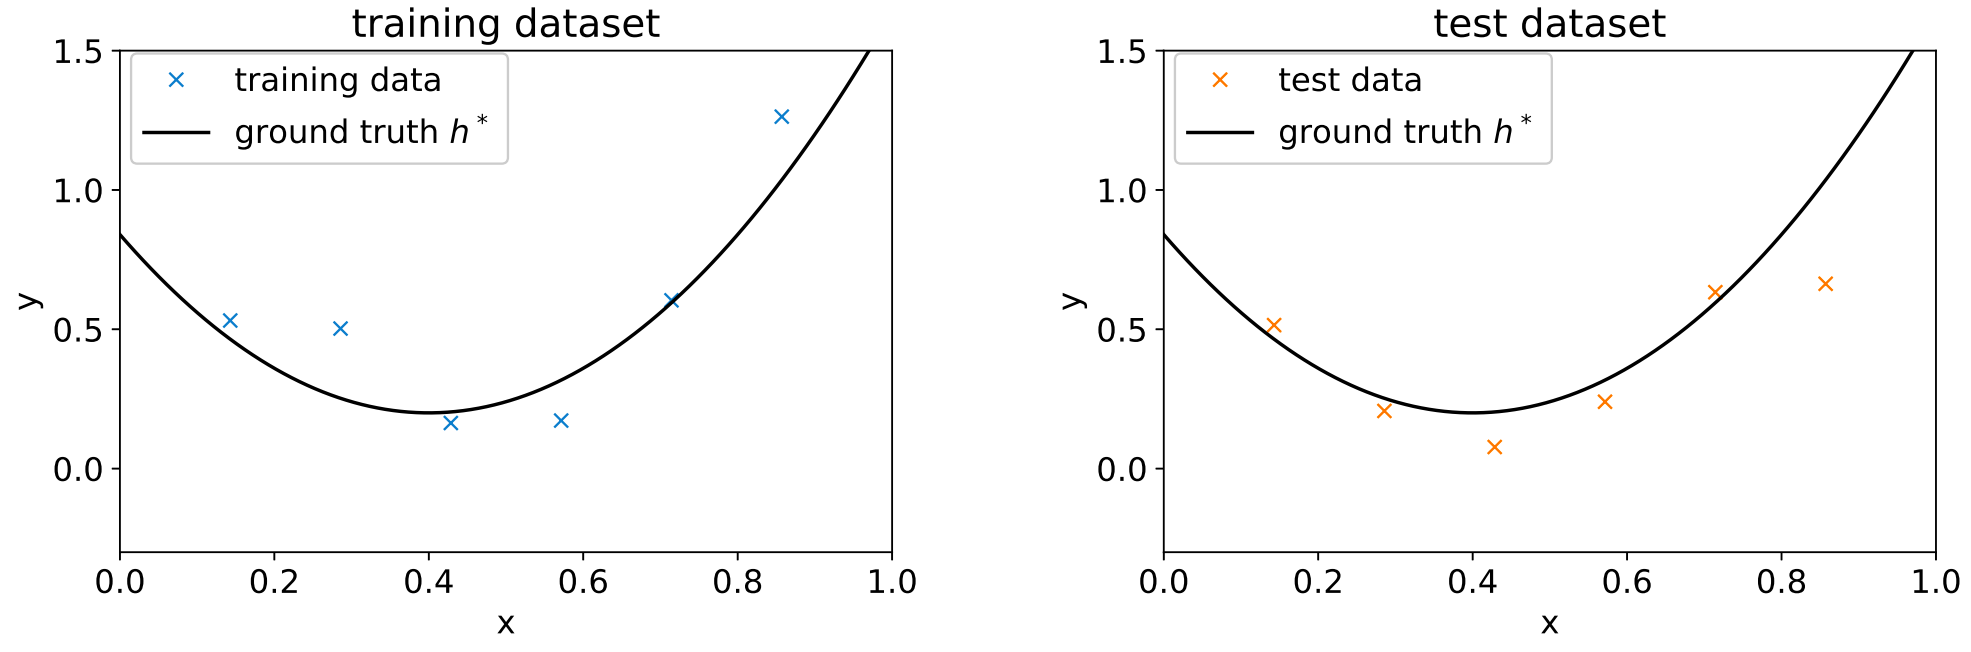
\includegraphics[width=0.8\linewidth]{figs/fitting_gt.png}
    \caption{用于本节的一个训练数据集和测试数据集的示例}
    \label{fig:8.1}
\end{figure}

作为说明性示例,考虑图 \ref{fig:8.1} 所示的训练数据集和测试数据集。训练输入 $x^{(i)}$ 是随机选择的,输出 $y^{(i)}$ 由 $y^{(i)} = h^*(x^{(i)}) + \xi^{(i)}$ 生成,其中函数 $h^*(\cdot)$ 是一个二次函数,在图 \ref{fig:8.1} 中以实线显示,而 $\xi^{(i)}$ 是假定从 $\sim N(0, \sigma^2)$ 生成的观测噪声。测试样本 $(x, y)$ 也有相同的输入-输出关系 $y = h^*(x) + \xi$,其中 $\xi \sim N(0, \sigma^2)$。预测噪声 $\xi$ 是不可能的,因此本质上我们的目标是恢复函数 $h^*(\cdot)$。

将考虑学习各种类型模型的测试误差。在讨论线性回归时,讨论了拟合“简单”模型,例如线性模型 $y = \theta_0 + \theta_1 x$,还是更“复杂”的模型,例如多项式模型 $y = \theta_0 + \theta_1 x + \dots + \theta_5 x^5$ 的问题。

从拟合线性模型开始,如图 \ref{fig:8.2} 所示。即使在训练数据集上,最佳拟合线性模型也无法准确预测 $y$ 与 $x$ 的关系,更不用说在测试数据集上了。这是因为 $y$ 和 $x$ 之间的真实关系不是线性的——任何线性模型都远离真实函数 $h^*(\cdot)$。因此,训练误差很大,这是\textit{欠拟合}的典型情况。

\begin{figure}[H]
    \centering
    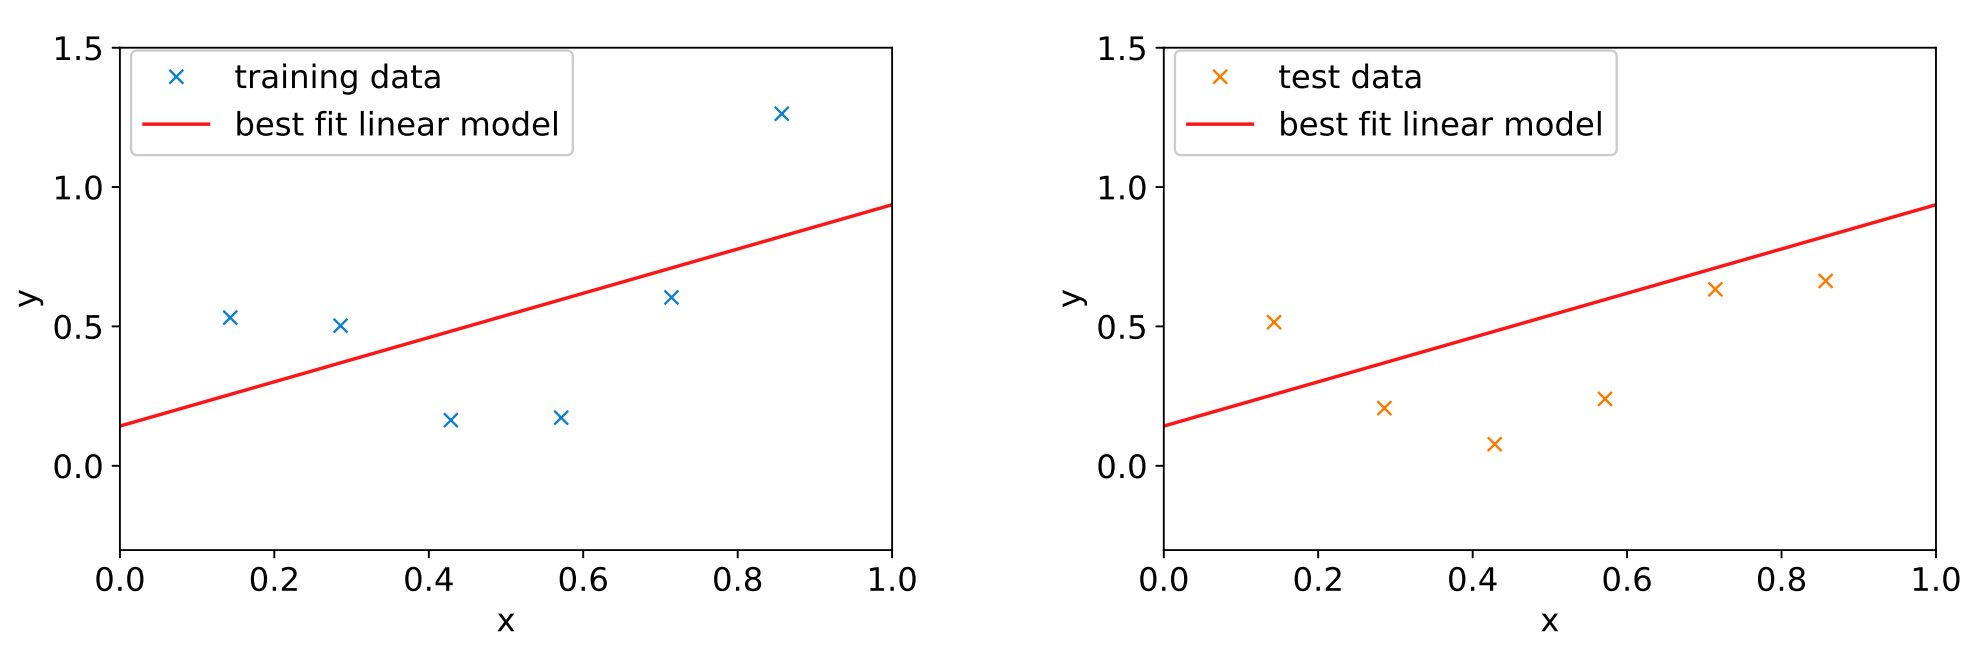
\includegraphics[width=0.8\linewidth]{figs/fitting_linear.png}
    \caption{最好的线性拟合模型也有着巨大的训练和测试误差。}
    \label{fig:8.2}
\end{figure}

\begin{figure}[H]
    \centering
    \begin{minipage}{0.475\linewidth}
        \centering
        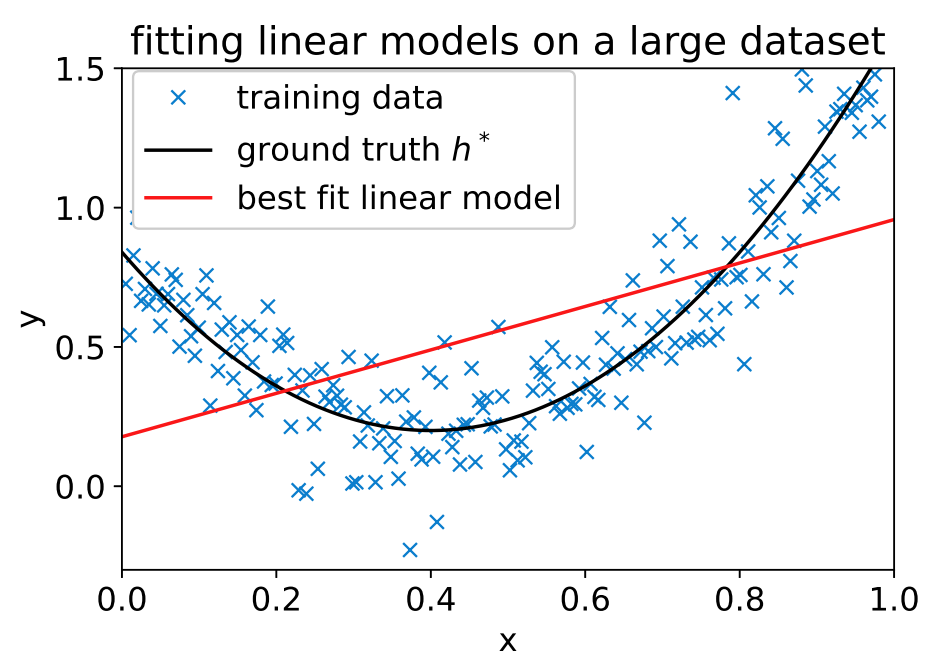
\includegraphics[{width=0.85\linewidth}]{figs/fitting_large.png}
        \caption{最好的线性拟合模型在超大训练集上也有着巨大的训练误差。}
        \label{fig:8.3}
    \end{minipage}\quad
    \begin{minipage}{0.475\linewidth}
        \centering
        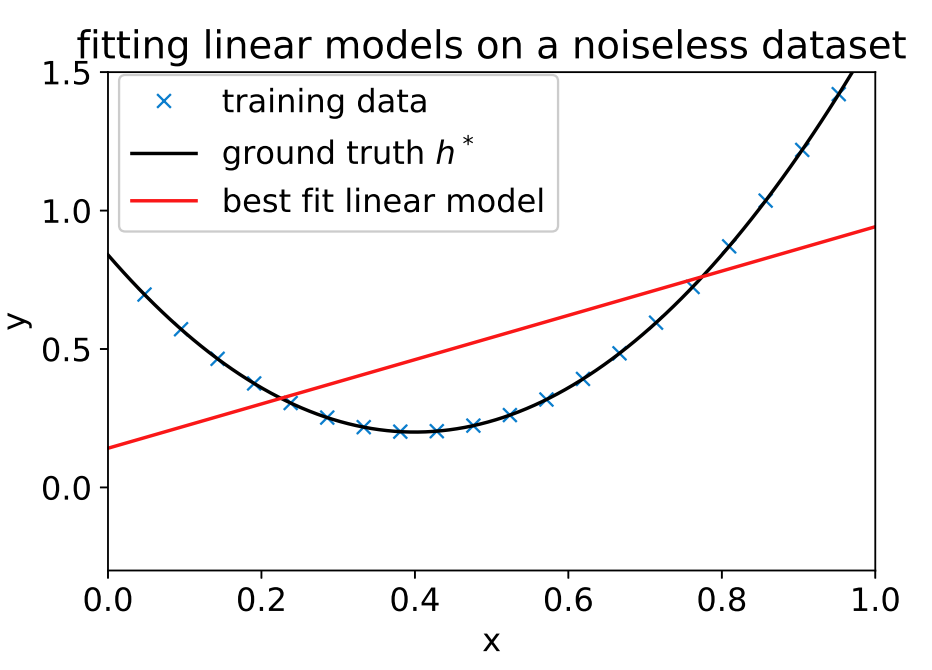
\includegraphics[width=0.85\linewidth]{figs/fitting_noiseless.png}
        \caption{最好的线性拟合模型在没有噪声的训练集上也有着巨大的训练和测试误差。}
        \label{fig:8.4}
    \end{minipage}
\end{figure}

这个问题不能通过增加训练样本来缓解——即使有非常大量的,甚至无限的训练样本,最佳拟合的线性模型仍然不准确,并且无法捕捉数据的结构(图 \ref{fig:8.3})。即使训练数据中不存在噪声,问题仍然存在(图 \ref{fig:8.4})。因此,这里的根本瓶颈在于线性模型族无法捕捉数据中的结构——线性模型无法表示真实的二次函数 $h^*$——而不是缺乏数据。非正式地,我们将模型的\textbf{偏差 (bias)} 定义为即使我们将其拟合到非常大(例如,无限大)的训练数据集时的测试误差。因此,在这种情况下,线性模型具有较大的偏差,并且欠拟合(即无法捕捉数据所表现出的结构)。

接下来,我们将一个 5 次多项式拟合到数据。图 \ref{fig:8.5} 表明它也未能学习到一个好的模型。然而,其失败模式与线性模型的情况不同。具体来说,尽管学习到的 5 次多项式在预测训练样本的 $y^{(i)}$ 与 $x^{(i)}$ 时表现非常好,但在测试样本上效果不佳(图 \ref{fig:8.5})。换句话说,从训练集学习到的模型无法很好地\textit{泛化 (generalize)} 到其他测试样本——测试误差很高。与线性模型的行为相反,5 次多项式的偏差较小——如果我们将 5 次多项式拟合到非常大的数据集,得到的模型将接近二次函数并且也很准确(图 \ref{fig:8.6})。这是因为 5 次多项式族包含所有二次函数(将 $\theta_5 = \theta_4 = \theta_3 = 0$ 设置为零即可得到二次函数),因此,原则上 5 次多项式能够捕捉数据的结构。

\begin{figure}[H]
    \centering
    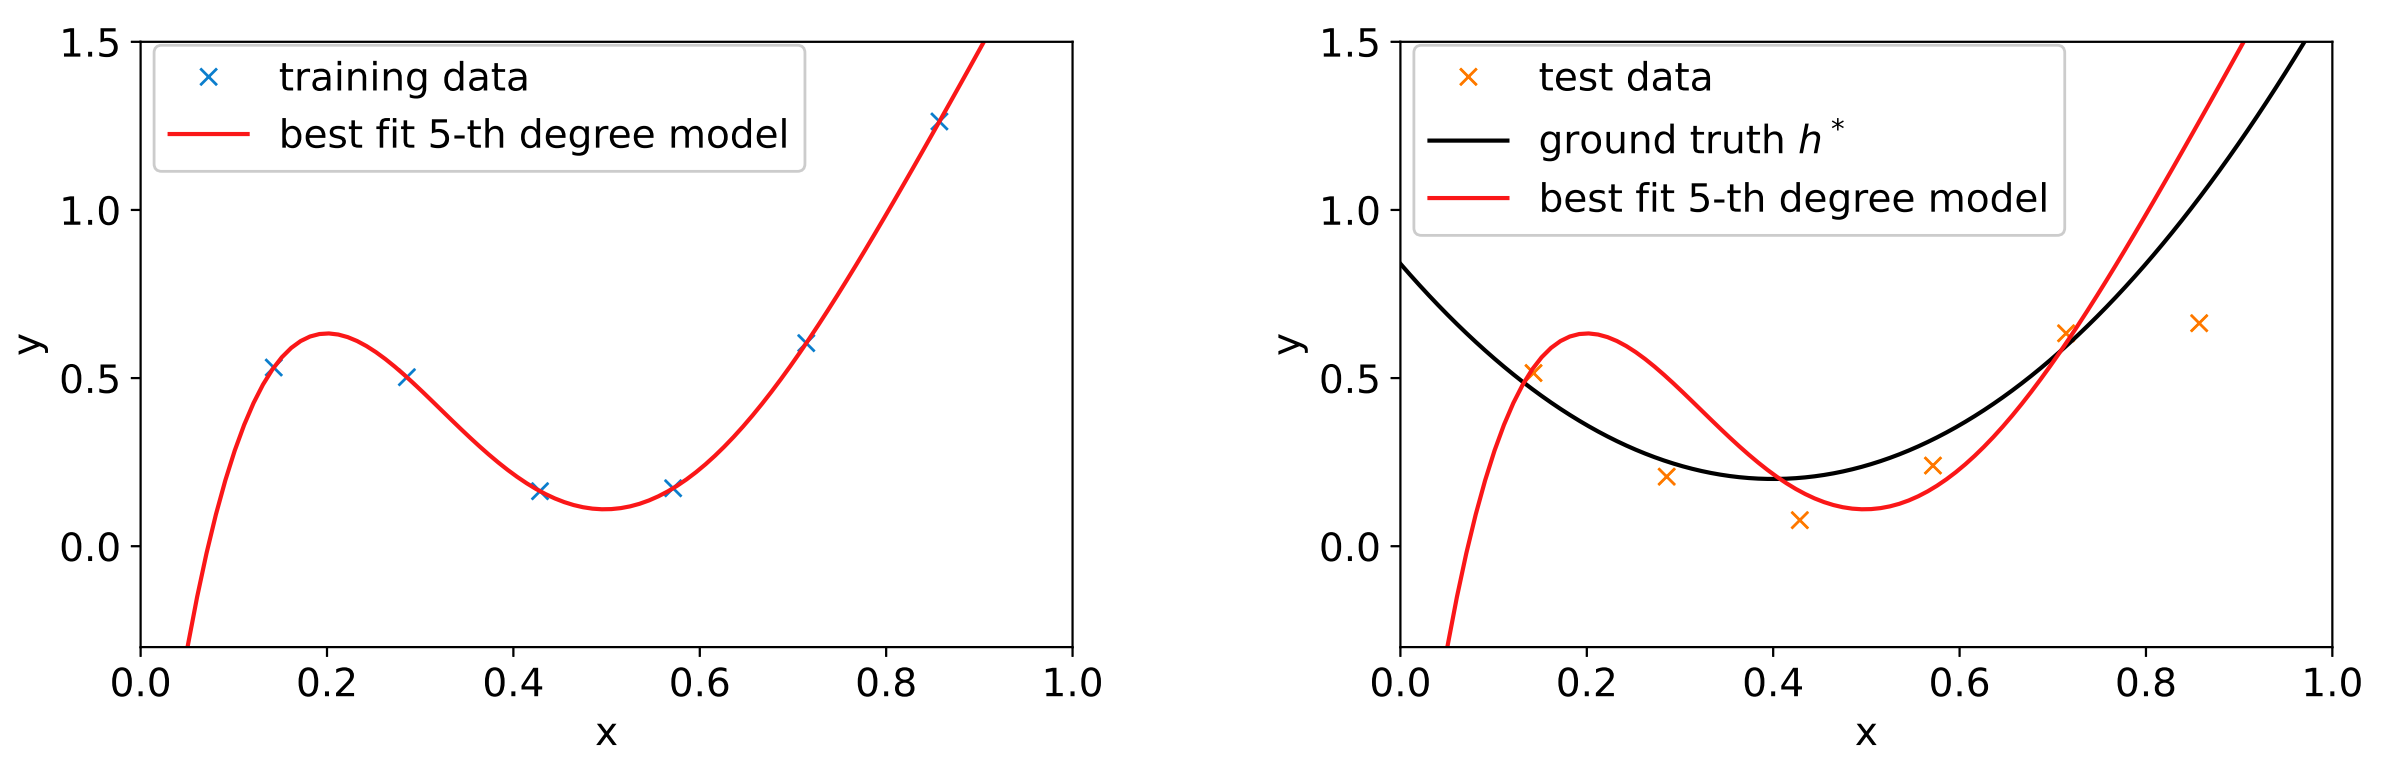
\includegraphics[width=0.8\linewidth]{figs/fitting_5th.png}
    \caption{最佳的 5 次多项式拟合模型训练误差为零,但测试误差仍然很大,并且未能恢复真实情况。这是经典的过拟合情形。}
    \label{fig:8.5}
\end{figure}

\begin{figure}[H]
    \centering
    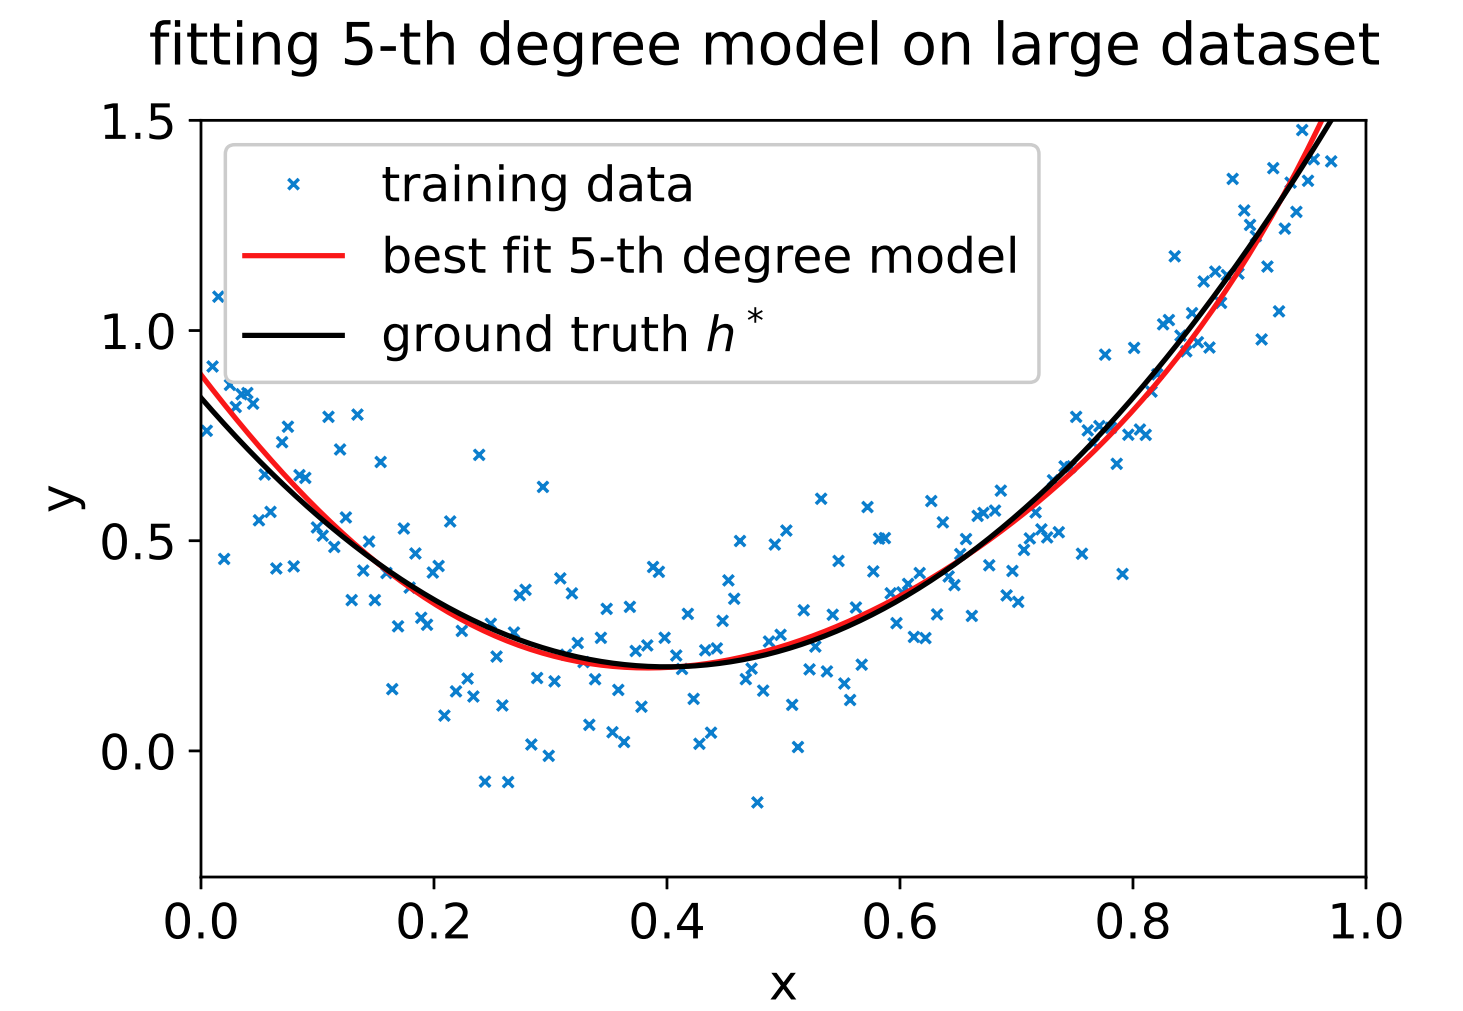
\includegraphics[width=0.5\linewidth]{figs/fitting_5th_large.png}
    \caption{在大型数据集上拟合的最佳 5 次多项式几乎恢复了真实情况——这表明图 \ref{fig:8.5} 中的问题是方差(或数据不足)而不是偏差。}
    \label{fig:8.6}
\end{figure}

拟合 5 次多项式的失败可以用测试误差的另一个组成部分来解释,称为模型拟合过程的\textbf{方差 (variance)}。具体来说,如图 \ref{fig:8.7} 所示,在拟合 5 次多项式时,存在很大的风险,即我们拟合了数据中恰好存在于我们\textit{小而有限 (small, finite)} 的训练集中的模式,但这些模式并不能反映 $x$ 和 $y$ 之间关系的更广泛模式。训练集中的这些“虚假”模式(大部分)是由于观测噪声 $\xi^{(i)}$ 引起的,拟合这些虚假模式会导致模型具有较大的测试误差。在这种情况下,我们称模型具有较大的方差。

\begin{figure}[H]
    \centering
    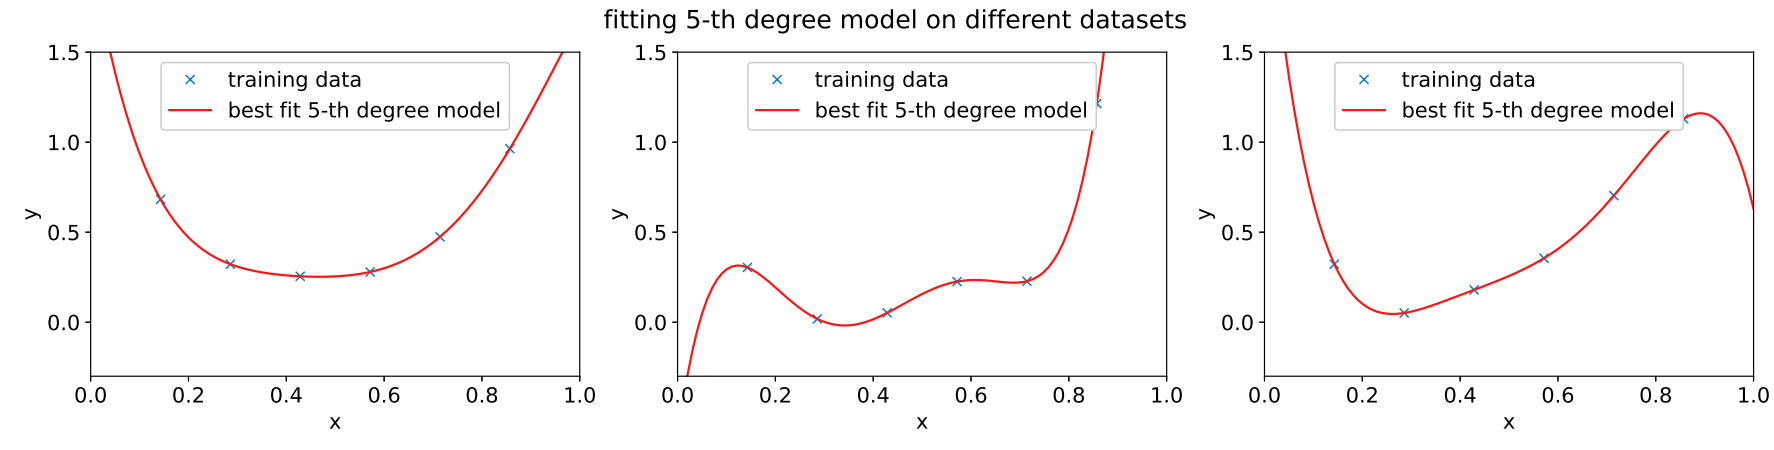
\includegraphics[width=0.95\linewidth]{figs/fitting_5th_different.png}
    \caption{在三个从同一分布产生的不同数据集上拟合的最佳 5 次多项式表现出极大不同,揭示其存在的巨大方差。}
    \label{fig:8.7}
\end{figure}

方差可以直观地(以及数学上证明,如第 \ref{sec:8.1.1} 节所示)通过在多个不同的训练数据集(从相同的潜在分布中抽取)上学习到的模型之间的变化量来表征。“虚假模式”是特定于特定数据集中的噪声(和输入)的随机性,因此在多个训练数据集之间是不同的。因此,对多个数据集的“虚假模式”过拟合应该会导致非常不同的模型。实际上,如图 \ref{fig:8.7} 所示,在三个不同训练数据集上学习到的模型差异很大,对每个数据集的“虚假模式”都存在过拟合。通常,偏差和方差之间存在权衡。如果我们的模型过于“简单”且参数很少,那么它可能具有较大的偏差(但方差较小),并且通常会遭受欠拟合。如果它过于“复杂”且参数很多,那么它可能遭受较大的方差(但偏差较小),因此会过拟合。图 \ref{fig:8.8} 展示了偏差和方差之间典型的权衡关系。

\begin{figure}[H]
    \centering
    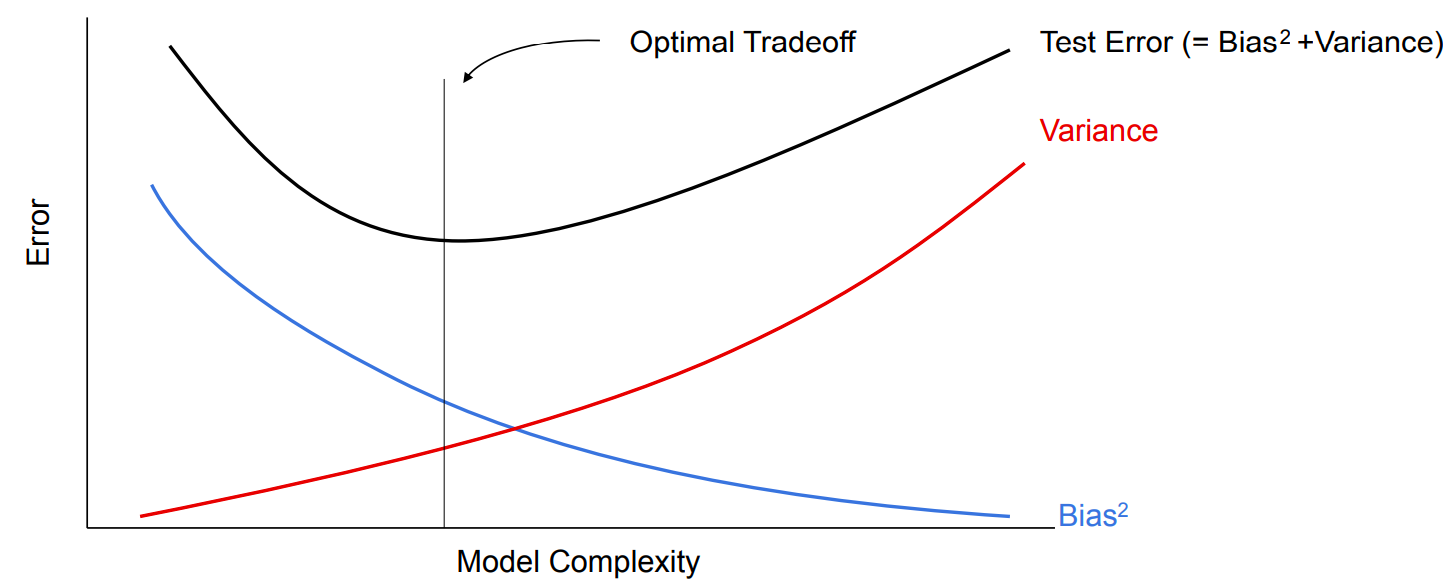
\includegraphics[width=0.9\linewidth]{figs/bias-variance_tradeoff.png}
    \caption{典型的偏差-方差权衡示意图。}
    \label{fig:8.8}
\end{figure}

正如我们将在第 \ref{sec:8.1.1} 节中正式看到的,测试误差可以分解为偏差和方差之和。这意味着随着模型复杂度的增加,测试误差将呈现凸曲线,在实践中我们应该调整模型复杂度以达到最佳权衡。例如,在上面的例子中,拟合二次函数比拟合一次或五次多项式效果更好,如图 \ref{fig:8.9} 所示。

\begin{figure}[H]
    \centering
    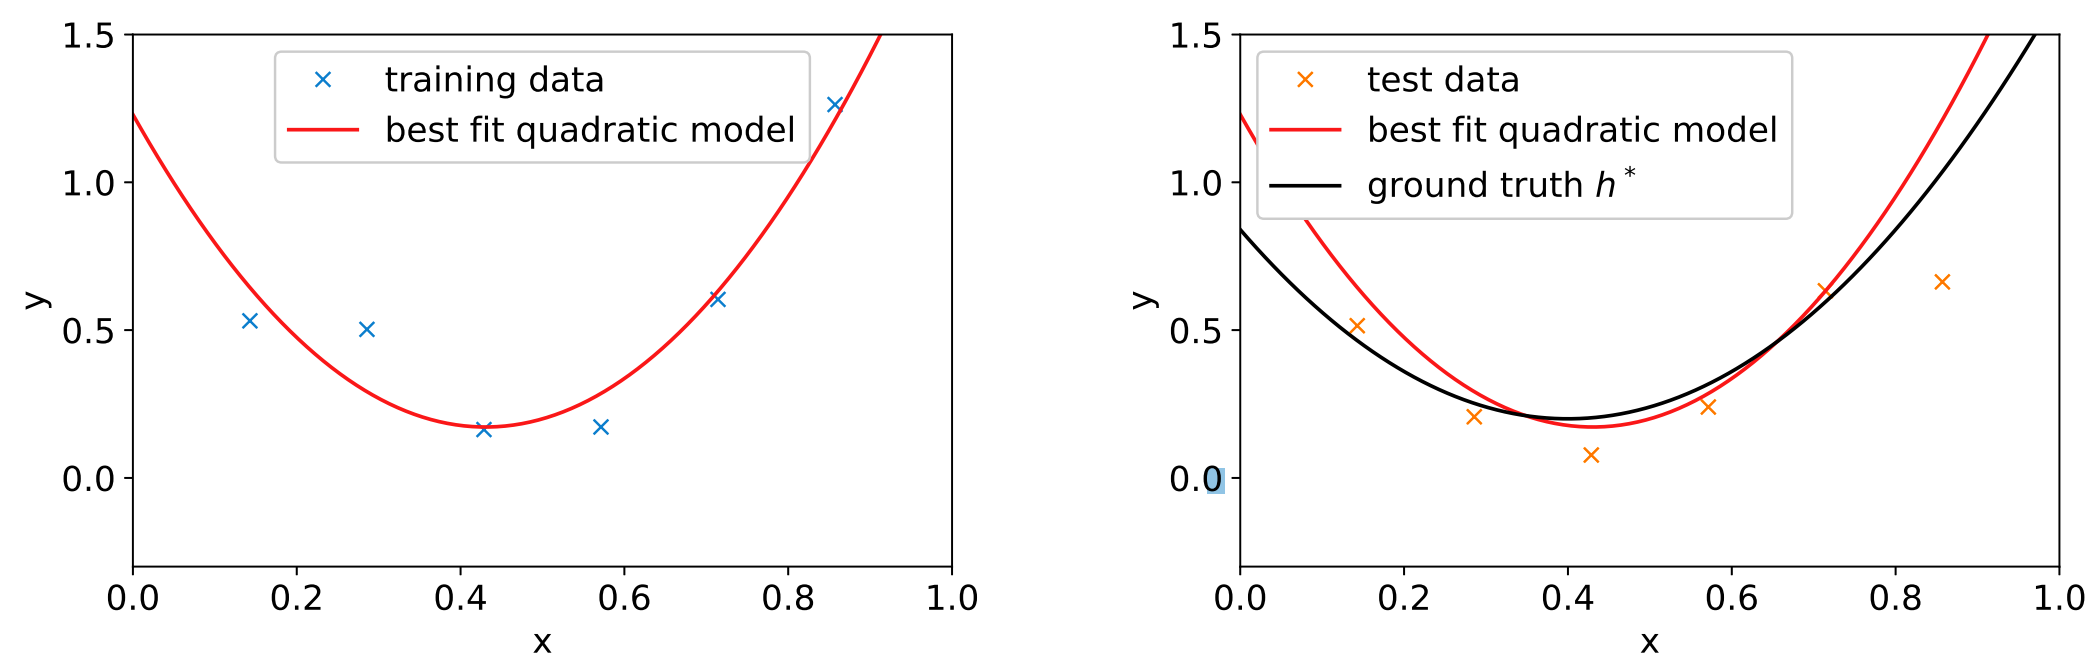
\includegraphics[width=0.8\linewidth]{figs/fitting_quadratic.png}
    \caption{最佳的二次拟合模型的训练误差和测试误差都很小,因为二次模型达到了良好的偏差-方差权衡。}
    \label{fig:8.9}
\end{figure}

有趣的是,偏差-方差权衡曲线或测试误差曲线并不普遍遵循图 \ref{fig:8.8} 中的形状,至少当模型复杂度仅通过参数数量衡量时并非如此。(我们将在 \ref{sec:8.2} 节中讨论所谓的双下降现象。)尽管如此,偏差-方差权衡原理在分析和预测测试误差的行为时,可能仍然是首选方法。

\subsection{(对于回归问题的)数学分解}\label{sec:8.1.1}

为了形式化回归问题的偏差-方差权衡,我们考虑如下设置(这是 \ref{sec:8.1} 节开头段落的扩展)
\begin{itemize}
    \item 抽取一个训练数据集 $S = \{x^{(i)}, y^{(i)}\}_{i=1}^n$,其中 $y^{(i)} = h^*(x^{(i)}) + \xi^{(i)}$ 且 $\xi^{(i)} \in N(0, \sigma^2)$。
    \item 在数据集 $S$ 上训练一个模型,记为 $\hat{h}_S$。
    \item 取一个测试样本 $(x, y)$,使得 $y = h^*(x) + \xi$ 且 $\xi \sim N(0, \sigma^2)$,并测量测试误差的期望(在随机抽取的训练集 $S$ 和随机的 $\xi$ 上进行平均)。\footnote{为简单起见,这里测试输入 $x$ 被视为固定,但在对 $x$ 进行平均时,同样的思想仍然成立。}\footnote{期望符号下的下标是为了强调在期望运算中被视为随机的变量。}
    \begin{equation}
        \text{MSE}(x) = \mathbb{E}_{S, \xi}[(y - \hat{h}_S(x))^2] \label{eq:8.2}
    \end{equation}
\end{itemize}

我们将把 MSE 分解为偏差项和方差项。我们从一个简单的数学工具开始,该工具将在下面使用两次。

\begin{claim}\label{claim:8.1.1}
    假设 $A$ 和 $B$ 是两个独立的实随机变量,且 $\mathbb{E}[A] = 0$。则 $\mathbb{E}[(A + B)^2] = \mathbb{E}[A^2] + \mathbb{E}[B^2]$。\\
    推论:因为随机变量 $A$ 与常数 $c$ 独立,当 $\mathbb{E}[A] = 0$ 时,我们有 $\mathbb{E}[(A+c)^2] = \mathbb{E}[A^2] + c^2$。
\end{claim}

断言的证明通过展开平方项得出:$\mathbb{E}[(A + B)^2] = \mathbb{E}[A^2 + B^2 + 2AB] = \mathbb{E}[A^2] + \mathbb{E}[B^2] + 2\mathbb{E}[AB] = \mathbb{E}[A^2] + \mathbb{E}[B^2]$。这里我们使用了独立性来证明 $\mathbb{E}[AB] = \mathbb{E}[A]\mathbb{E}[B] = 0$。
使用断言 \ref{claim:8.1.1},令 $A = \xi$ 且 $B = h^*(x) - \hat{h}_S(x)$,我们有
\begin{align}
    \text{MSE}(x) = \mathbb{E}[(y - \hat{h}_S(x))^2] &= \mathbb{E}[(\xi + (h^*(x) - \hat{h}_S(x)))^2] \label{eq:8.3} \\
    &= \mathbb{E}[\xi^2] + \mathbb{E}[(h^*(x) - \hat{h}_S(x))^2] \quad (\text{根据断言 \ref{claim:8.1.1}})  \nonumber\\
    &= \sigma^2 + \mathbb{E}[(h^*(x) - \hat{h}_S(x))^2] \label{eq:8.4}
\end{align}

然后,我们定义 $h_{\text{avg}}(x) = \mathbb{E}_S[\hat{h}_S(x)]$ 为“平均模型”——通过抽取无限多个数据集,并在其上进行训练,然后对它们在 $x$ 上的预测进行平均而获得的模型。注意,$h_{\text{avg}}$ 是一个用于分析目的的假设模型,它在现实中无法获得(因为我们无法拥有无限多个数据集)。结果表明,对于许多情况,$h_{\text{avg}}$(近似)等于在具有无限样本的单个数据集上训练得到的模型。因此,我们也可以直观地解释 $h_{\text{avg}}$,这与我们在上一小节中对偏差的直观定义一致。

我们可以通过令 $c = h^*(x) - h_{\text{avg}}(x)$(这是一个不依赖于 $S$ 选择的常数)和 $A = h_{\text{avg}}(x) - \hat{h}_S(x)$ 来进一步分解 $\text{MSE}(x)$,这符合断言 \ref{claim:8.1.1} 的推论:
\begin{align}
    \text{MSE}(x) &= \sigma^2 + \mathbb{E}[(h^*(x) - \hat{h}_S(x))^2] \label{eq:8.5} \\
    &= \sigma^2 + \mathbb{E}[(h^*(x) - h_{\text{avg}}(x) + h_{\text{avg}}(x) - \hat{h}S(x))^2] \label{eq:8.6} \\
    &= \underbrace{\sigma^2}_{\text{不可避免}} + \underbrace{(h^*(x) - h_{\text{avg}}(x))^2}_{\text{偏差}^2} + \underbrace{\text{var}(\hat{h}S(x))}_{\text{方差}} \label{eq:8.7}
\end{align}
我们将第二项称为偏差(平方),第三项称为方差。如前所述,偏差捕捉了由于模型表达能力不足而引入的误差部分。回想一下,$h_{\text{avg}}$ 可以被认为是即使在无限数据下学习到的最佳可能模型。因此,偏差并非根本上由数据不足引起,而是由模型族本身无法很好地近似 $h^*$ 造成的。例如,在图 \ref{fig:8.2} 所示的例子中,由于任何线性模型都无法近似真实的二次函数 $h^*$,因此 $h_{\text{avg}}$ 也不能,从而偏差项很大。
方差项捕捉了有限数据集的随机性如何引入学习模型中的误差。它衡量了学习模型对数据集中随机性的敏感度。随着数据集大小的增加,方差通常会减小。
对于第一项 $\sigma^2$,我们无能为力,因为根据定义,我们无法预测噪声 $\xi$。
最后,我们注意到,分类问题的偏差-方差分解远不如回归问题清晰。已经有一些提案,但对于什么是“正确”和/或最有用的形式还没有达成一致。


\section{双下降现象}\label{sec:8.2}

\subsection*{模型层面的双下降现象}

最近的研究表明,在包括线性模型和深度神经网络在内的一系列机器学习模型中,测试误差会呈现出一种“双下降”现象。\footnote{该现象的发现可能可以追溯到 \cite{opper1995statistical,opper2001learning},最近由 \cite{belkin2020two,hastie2022surprises} 推广。} 正如 \ref{sec:8.1} 节中所讨论的传统观点是,随着模型复杂度的增加,测试误差先下降然后上升,如图 \ref{fig:8.8} 所示。然而,在许多情况下,我们经验性地观察到测试误差可以有第二次下降——它先下降,然后在大到足以很好地拟合所有训练数据时达到峰值附近,然后在所谓的过参数化区域再次下降,其中参数数量大于数据点数量。图 \ref{fig:8.10} 展示了测试误差随模型复杂度(由参数数量衡量)变化的典型曲线。在某种程度上,过参数化区域的第二次下降被认为是机器学习领域的新发现——部分原因是轻度正则化的过参数化模型在深度学习时代得到了广泛应用。这种现象的一个实际意义是,不应回避扩大模型规模和尝试过参数化模型,因为测试误差很可能再次下降到比之前的最低点更低的水平。实际上,在许多情况下,更大的过参数化模型总是能带来更好的测试性能(这意味着第二次下降之后不会出现第二次上升)。

\begin{figure}[H]
    \centering
    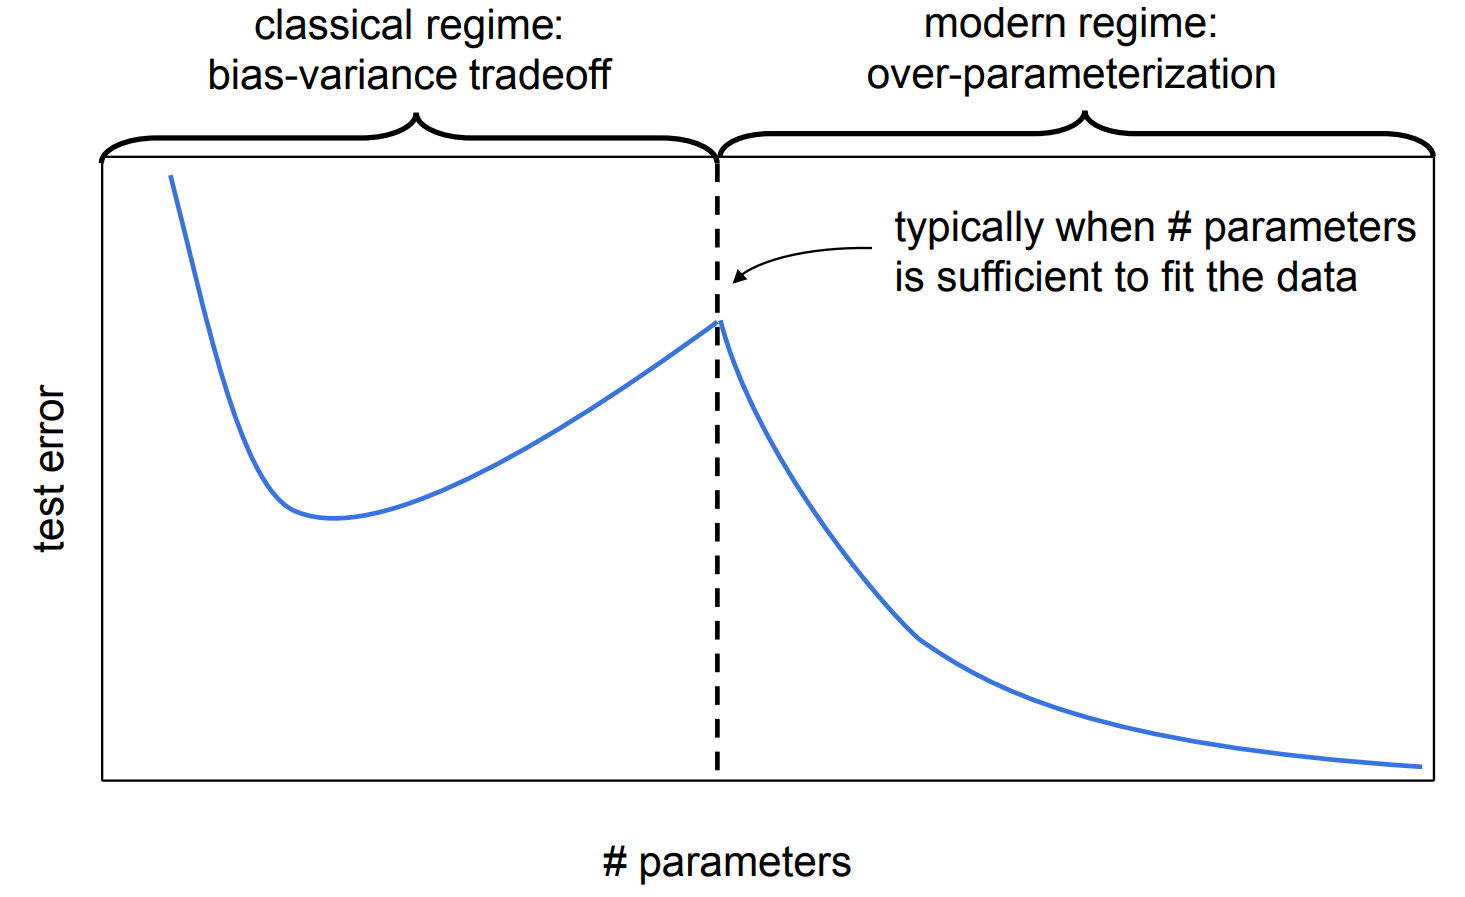
\includegraphics[width=0.8\linewidth]{figs/double_descent.png}
    \caption{典型的模型层面双下降现象。随着参数数量的增加,当参数数量小于训练数据时,测试误差先下降。然后在过参数化区域,测试误差再次下降。}
    \label{fig:8.10}
\end{figure}

\subsection*{样本层面的双下降现象}

从先验知识来看,我们期望更多的训练样本总是能带来更小的测试误差——更多的样本为算法提供了更严格的信息来学习。然而,最近的研究 [\cite{nakkiran2019more}] 观察到,随着样本数量的增加,测试误差并非单调递减。相反,如图 \ref{fig:8.11} 所示,测试误差先下降,然后在样本数量(记为 $n$)与参数数量(记为 $d$)接近时增加并达到峰值,然后再次下降。我们将此称为样本层面的双下降现象。在某种程度上,样本层面的双下降和模型层面的双下降本质上描述的是类似的现象——测试误差在 $n \approx d$ 时达到峰值。

\begin{figure}[H]
    \centering
    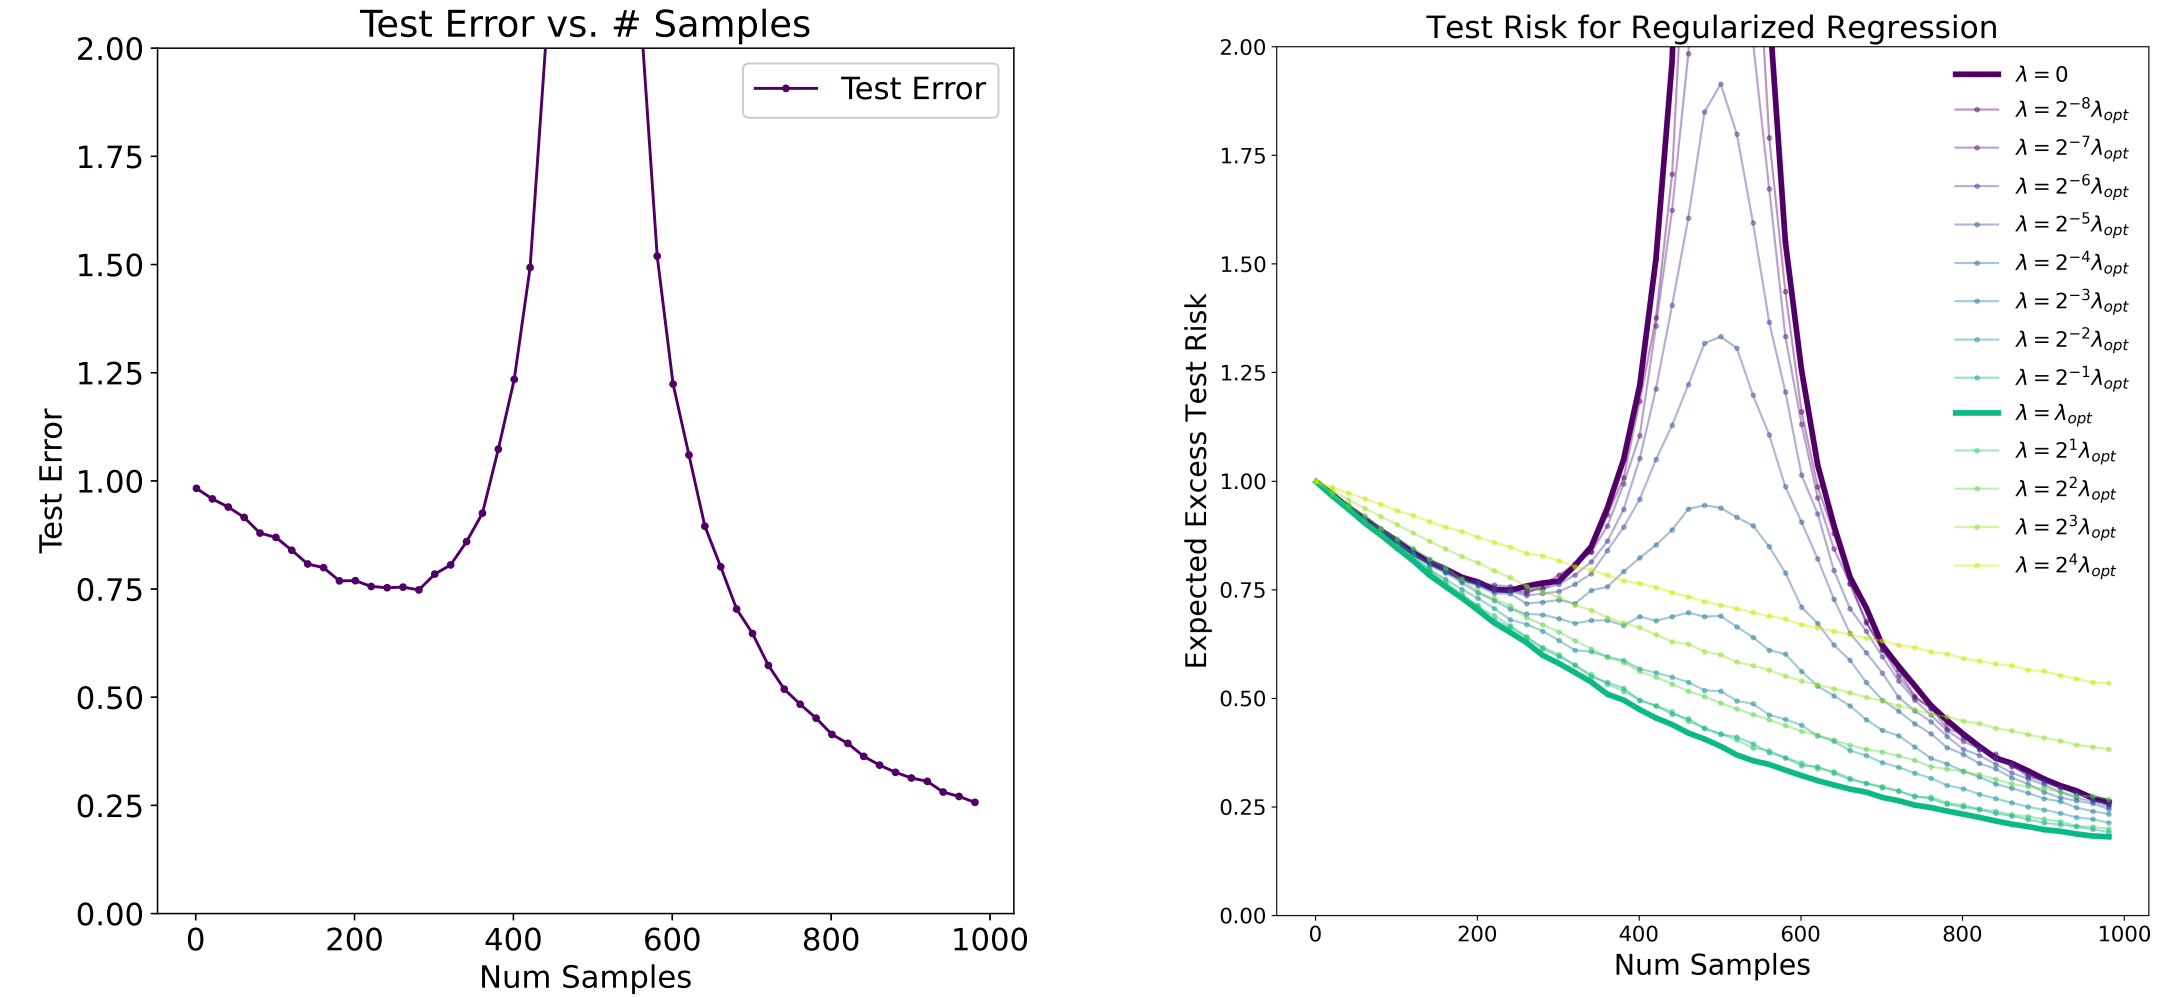
\includegraphics[width=0.9\linewidth]{figs/sample_double_descent.png}
    \caption{\textbf{左:}线性模型在样本层面的双下降现象。\textbf{右:}不同正则化强度下线性模型在样本层面的双下降现象。 使用最优正则化参数(对每个 $n$ 都调到最优,以绿色实线显示)缓解双下降。 \textbf{设置:}$(x, y)$ 的数据分布为 $x \sim \mathcal{N}(0, I_d)$ 且 $y \sim x^\top \beta + \mathcal{N}(0, \sigma^2)$,其中 $d = 500$, $\sigma = 0.5$ 且 $\|\beta\|_2 = 1$.\protect\footnotemark}
    \label{fig:8.11}
\end{figure}
\footnotetext[8]{此图依照 \cite{nakkiran2020optimal} 的图 1 复现,类似的现象也可以在 \cite{hastie2022surprises,mei2022generalization} 中观察到。}

\subsection*{解释和缓解策略}

样本层面的双下降,特别是测试误差在 $n \approx d$ 处的峰值,表明在这些实验中评估的现有训练算法在 $n \approx d$ 时远非最优。我们可以通过丢弃一些样本,使用较小的样本量运行算法来避免峰值。换句话说,原则上存在其他算法可以在 $n \approx d$ 时实现更小的测试误差,但这些实验中评估的算法未能做到。学习过程的次优性似乎是样本层面和模型层面双下降峰值的罪魁祸首。
实际上,通过最优调整的正则化(将在第 \ref{chapter:9} 章中更详细讨论),在 $n \approx d$ 区域的测试误差可以显著改善,并且模型层面和样本层面的双下降现象都得到了缓解。参见图 \ref{fig:8.11}。
上述直觉只解释了模型层面和样本层面双下降的峰值,但没有解释模型层面双下降的第二次下降——为什么过参数化模型能够很好地泛化。对过参数化模型的理论理解是一个活跃的研究领域,最近取得了许多进展。一个典型的解释是,常用的优化器(如梯度下降)提供了隐式正则化效应(将在第 \ref{sec:9.2} 节中更详细讨论)。换句话说,即使在过参数化区域且使用了非正则化的损失函数,模型仍然隐式地进行了正则化,因此表现出比拟合数据的任意解更好的测试性能。例如,对于线性模型,当 $n \ll d$ 时,使用零初始化进行梯度下降的优化器会找到拟合数据的\textit{最小范数 (minimum norm)} 解(而不是拟合数据的任意解),而最小范数正则化器对于过参数化区域来说是一个足够好的正则化器(但在 $n \approx d$ 时不是一个好的正则化器,导致测试误差达到峰值)。

\begin{figure}[H]
    \centering
    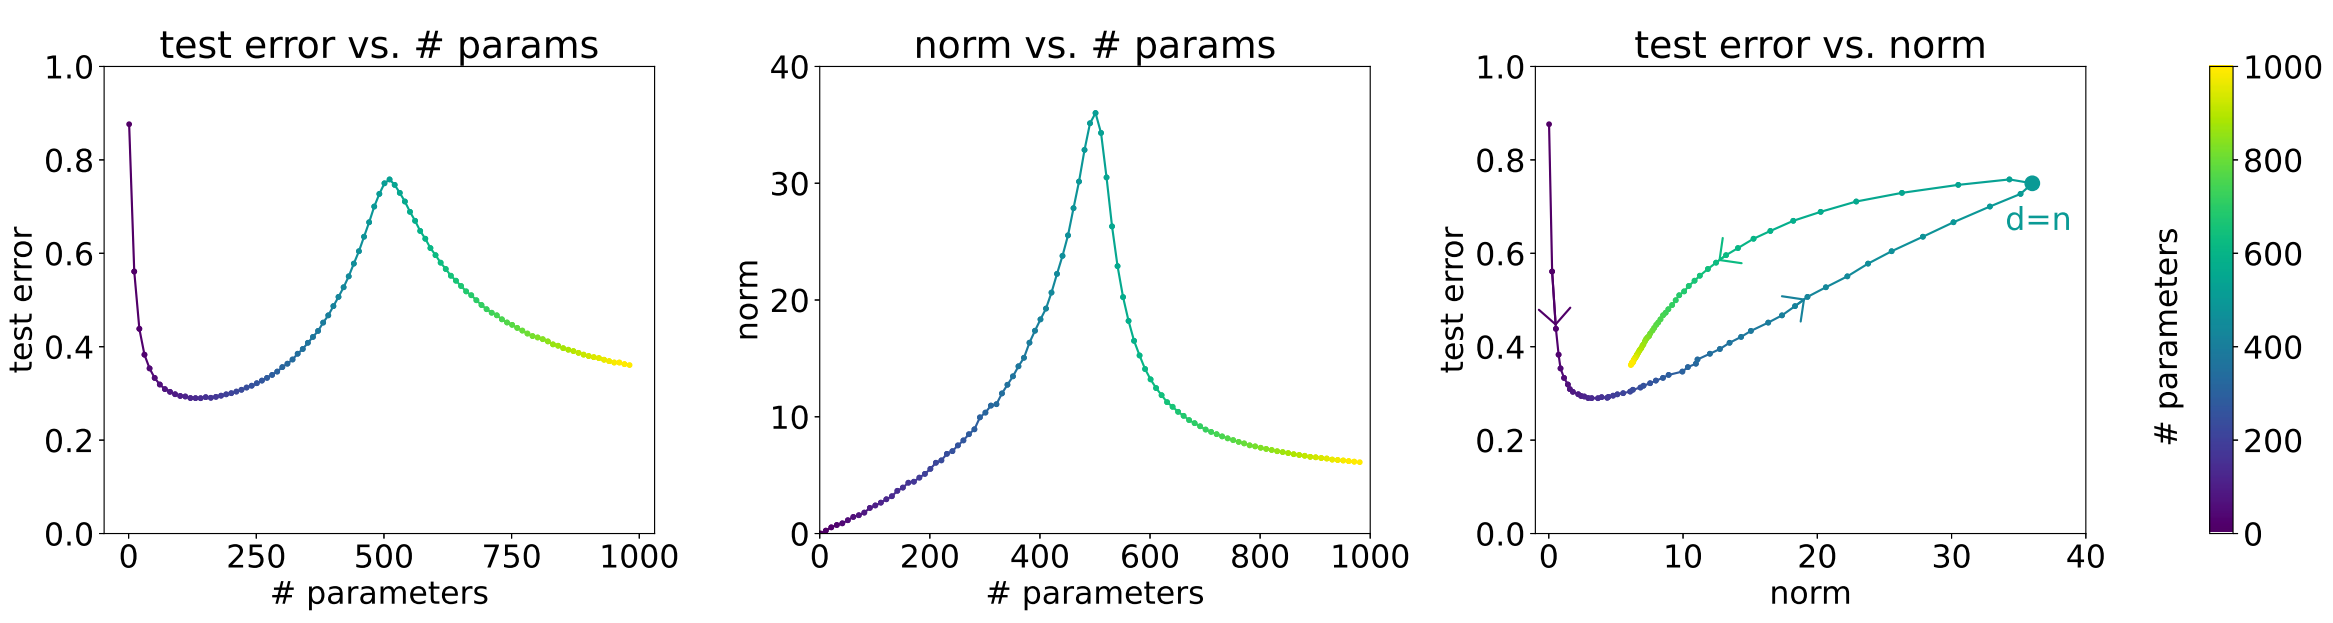
\includegraphics[width=1.0\linewidth]{figs/double_descent_norm.png}
    \caption{\textbf{左:}双下降现象,其中模型复杂度用参数数量来衡量。\textbf{中:}学习到的模型的范数在 $n \approx d$ 附近达到峰值。\textbf{右:}测试误差与学习到的模型范数的关系。颜色条表示参数数量,箭头表示模型尺寸增加的方向。它们的关系更接近于传统认知,而不是双下降。 \textbf{设置}:我们考虑一个样本量固定为 $n = 500$ 的线性回归。输入 $x$ 是 Fashion-MNIST 上的随机 ReLU 特征,输出 $y \in \mathbb{R}^{10}$ 是 one-hot 标签。这与 \cite{nakkiran2020optimal} 第 5.2 节中的设置相同。}
    \label{fig:8.12}
\end{figure}

最后,我们还要指出,双下降现象主要在模型的复杂度用参数数量来衡量时被观察到。参数数量是否以及何时是衡量模型复杂度的最佳指标尚不清楚。例如,在许多情况下,模型的范数被用作复杂度度量。如图 \ref{fig:8.12} 右图所示,对于一个特定的线性情况,如果我们绘制测试误差与学习到的模型范数的关系,双下降现象就不再发生。这部分是因为学习到的模型的范数在 $n \approx d$ 附近也达到峰值(参见图 \ref{fig:8.12}(中)或 \cite{belkin2019reconciling}、\cite{mei2022generalization},以及 \cite{james2021introduction} 在第 10.8 节中的讨论)。对于深度神经网络,正确的复杂度度量更加难以捉摸。双下降现象的研究仍是一个活跃的研究课题。

\section{样本复杂度边界 (选读)}\label{sec:8.3}
\subsection{预备知识}

在本节中,我们将开始探索学习理论。除了其本身具有的趣味性和启发性之外,本节的讨论还将帮助我们锻炼直觉,并推导如何在不同情境下最优地应用学习算法的经验法则。我们还将尝试回答几个关键问题:首先,我们能否形式化地描述刚刚讨论的偏差/方差权衡?这将最终引导我们讨论模型选择方法,例如,它可以自动决定将多项式拟合到训练集的阶数。其次,在机器学习中,我们真正关心的是泛化误差,但大多数学习算法是根据训练集来拟合模型的。为什么在训练集上表现良好能说明泛化误差方面的问题呢?具体来说,我们能否将训练集上的误差与泛化误差联系起来?第三也是最后一个问题,是否存在一些条件,在这些条件下我们可以实际证明学习算法是有效的?

我们先两个简单但非常有用的引理开始。

\begin{lemma*}
    (并集上界)
    设 $A_1, A_2, \dots, A_k$ 是 $k$ 个不同的事件(它们可能不相互独立)。那么
    \[
        P(A_1 \cup \dots \cup A_k) \leq P(A_1) + \dots + P(A_k).
    \]
\end{lemma*}

在概率论中,并集上界通常被视为公理(因此我们不尝试证明它),但它也具有直观意义:$k$ 个事件中任意一个发生的概率至多是这 $k$ 个不同事件的概率之和。

\begin{lemma*}
    (Hoeffding 不等式)
    设 $Z_1, \dots, Z_n$ 是从 Bernoulli($\phi$) 分布中独立同分布 (iid) 抽取的随机变量。即 $P(Z_i = 1) = \phi$,且 $P(Z_i = 0) = 1 - \phi$。设 $\hat{\phi} = (1/n) \sum_{i=1}^n Z_i$ 是这些随机变量的均值,并任取 $\gamma > 0$ 并固定住。那么
    \[
        P(|\phi - \hat{\phi}| > \gamma) \leq 2\exp(-2\gamma^2 n).
    \]
\end{lemma*}

这个引理(在学习理论中也称为 \textbf{Chernoff 界 (Chernoff bound)}) 表明,如果我们取 $\hat{\phi}$ 作为 $n$ 个 Bernoulli($\phi$) 随机变量的平均值来估计 $\phi$ 的真值,那么我们的估计值与真值相差很大的概率会很小,只要 $n$ 足够大。换句话说,如果你有一个抛出正面的概率为 $\phi$ 的有偏硬币,那么如果你抛掷 $n$ 次,计算出现正面的比例。当 $n$ 很大的时候,这大概率是 $\phi$ 的一个很好的估计值。

利用这两个引理,我们将能够证明学习理论中一些深刻且重要的结果。

为了简化,我们将重点放在标签 $y \in \{0, 1\}$ 的二分类问题上。我们在这里讨论的内容可以推广到其他问题,包括回归和多分类问题。

假设我们有一个大小为 $n$ 的训练集 $S = \{(x^{(i)}, y^{(i)}); i = 1, \dots, n\}$,其中训练样本 $(x^{(i)}, y^{(i)})$ 是从概率分布 $\mathcal{D}$ 中独立同分布地抽取的。对于一个假设 $h$,我们将学习理论中的\textbf{训练误差 (training error)}(也称为\textbf{经验风险 (empirical risk)} 或\textbf{经验误差 (empirical error)})定义为
\[
    \hat{\varepsilon}(h) = \frac{1}{n} \sum_{i=1}^n {1}\{h(x^{(i)}) \neq y^{(i)}\}.
\]
这是 $h$ 错误分类的训练样本的比例。当我们要明确指出 $\hat{\varepsilon}(h)$ 对训练集 $S$ 的依赖性时,也可以将其写成 $\hat{\varepsilon}_S(h)$。我们还定义泛化误差为
\[
    \varepsilon(h) = P_{(x,y) \sim \mathcal{D}}(h(x) \neq y).
\]
也就是说,这是如果我们从分布 $\mathcal{D}$ 中抽取一个新的样本 $(x, y)$, $h$ 将其错误分类的概率。

请注意,我们假设训练数据是从我们将用于评估我们的假设的\textit{相同 (same)} 分布 $\mathcal{D}$ 中抽取的(在泛化误差的定义中)。这有时也被视为 \textbf{PAC} 假设中的一条。\footnote{PAC (Probably Approximately Correct) 代表“可能近似正确”,它是学习理论中大量结果得以证明的框架和假设集合。其中,训练和测试样本来自相同分布的假设以及训练样本独立抽取的假设是最重要的。}

考虑线性分类的设置,并令 $h_\theta(x) = {1}\{\theta^\top x \geq 0\}$。拟合参数 $\theta$ 的合理方法是什么?一种方法是尝试最小化训练误差,并选择
\[
    \hat{\theta} = \arg \min_\theta \hat{\varepsilon}(h_\theta).
\]
我们将这个过程称为\textbf{经验风险最小化 (empirical risk minimization, ERM)},学习算法的输出假设为 $\hat{h} = h_{\hat{\theta}}$。我们将 ERM 视为最“基本”的学习算法,并且这个算法也是本节的重点。(逻辑回归等算法也可以看作是经验风险最小化的近似。)

在学习理论的研究中,将假设的具体参数化以及决策边界是否线性的问题抽象出来将会很有帮助。我们定义学习算法使用的\textbf{假设类 (hypothesis class)} $\mathcal{H}$ 为其考虑的所有分类器集合。对于线性分类,$\mathcal{H} = \{h_\theta: h_\theta(x) = {1}\{\theta^\top x \geq 0\}, \theta \in \mathbb{R}^{d+1}\}$,也就是是所有在 $\mathcal{X}$(输入的域)上决策边界为线性的分类器的集合。更广泛地说,如果我们研究的是神经网络,那么我们可以令 $\mathcal{H}$ 是由某种神经网络结构表示的所有分类器的集合。

经验风险最小化现在可以被视为在函数空间 $\mathcal{H}$ 上的最小化问题,其中学习算法选择的假设是
\[
    \hat{h} = \arg \min_{h \in \mathcal{H}} \hat{\varepsilon}(h).
\]

\subsection{有限 \texorpdfstring{$\mathcal{H}$}{H} 的情况}

让我们首先考虑一个学习问题,其有一个有限的假设类 $\mathcal{H} = \{h_1, \dots, h_k\}$,包含 $k$ 个假设。因此,$\mathcal{H}$ 是从 $\mathcal{X}$ 到 $\{0, 1\}$ 的 $k$ 个函数的集合,经验风险最小化选择 $\hat{h}$ 为这些函数中训练误差最小的那个。

我们希望对 $\hat{h}$ 的泛化误差给出保证。我们的策略将分为两部分:首先,我们将证明 $\hat{\varepsilon}(h)$ 是对所有 $h$ 的 $\varepsilon(h)$ 的可靠估计。其次,我们将证明这隐含了 $\hat{h}$ 的泛化误差的上界。

取任意一个固定的 $h_i \in \mathcal{H}$。考虑一个伯努利随机变量 $Z$,其分布定义如下。我们将从分布 $\mathcal{D}$ 中抽取样本 $(x, y)$。然后,我们设置 $Z = {1}\{h_i(x) \neq y\}$。也就是说,我们将抽取一个样本,并让 $Z$ 表示 $h_i$ 是否将其错误分类。类似地,我们还定义 $Z_j = {1}\{h_i(x^{(j)}) \neq y^{(j)}\}$。由于我们的训练集是从 $\mathcal{D}$ 中独立同分布地抽取的, $Z$ 和 $Z_j$ 具有相同的分布。

我们看到,随机抽取样本被错误分类的概率——即 $\varepsilon(h_i)$——恰好是 $Z$(以及 $Z_j$)的期望值。此外,训练误差可以写成
\[
    \hat{\varepsilon}(h_i) = \frac{1}{n} \sum_{j=1}^n Z_j.
\]
因此,$\hat{\varepsilon}(h_i)$ 恰好是从均值为 $\varepsilon(h_i)$ 的伯努利分布中独立同分布地抽取的 $n$ 个随机变量 $Z_j$ 的均值。因此,我们可以应用 Hoeffding 不等式,得到
\[
    P(|\varepsilon(h_i) - \hat{\varepsilon}(h_i)| > \gamma) \leq 2 \exp(-2\gamma^2 n).
\]

这表明,对于我们特定的 $h_i$,训练误差将依概率收敛到泛化误差,假设 $n$ 很大。但我们不只是想保证 $\hat{\varepsilon}(h_i)$ 将依概率收敛到 $\varepsilon(h_i)$,对于某一个特定的 $h_i$。我们希望证明这对所有 $h \in \mathcal{H}$ 同时成立。为此,令 $A_i$ 表示事件 $|\varepsilon(h_i) - \hat{\varepsilon}(h_i)| > \gamma$。我们已经证明,对于任意特定的 $A_i$,有 $P(A_i) \leq 2 \exp(-2\gamma^2 n)$。因此,利用并集上界,我们有
\begin{align*}
    P(\exists h \in \mathcal{H}. |\varepsilon(h) - \hat{\varepsilon}(h)| > \gamma) 
    &= P(A_1 \cup \dots \cup A_k) \\
    & \leq \sum_{i=1}^k P(A_i) \\
    & \leq \sum_{i=1}^k 2 \exp(-2\gamma^2 n) \\
    & = 2k \exp(-2\gamma^2 n).
\end{align*}
如果用 1 中减去不等式两侧,可以发现
\begin{align*}
    P(\neg \exists h \in \mathcal{H}. |\varepsilon(h) - \hat{\varepsilon}(h)| > \gamma) 
    & = P(\forall h \in \mathcal{H}. |\varepsilon(h) - \hat{\varepsilon}(h)| \leq \gamma) \\
    & \geq 1 - 2k \exp(-2\gamma^2 n).
\end{align*}
(“$\neg$”符号表示“逻辑非”。)因此可以保证,对于所有 $h \in \mathcal{H}$,$\hat{\varepsilon}(h)$ 在 $\varepsilon(h)$ 的 $\gamma$ 范围内的概率不低于 $1 - 2k \exp(-2\gamma^2 n)$。这被称为\textit{一致收敛 (uniform convergence)} 结果,因为这是一个对所有(而不是单独一个)$h \in \mathcal{H}$ 同时成立的界。

在上面的讨论中,我们所做的,是对于特定的 $n$ 和 $\gamma$ 值,给出了某些 $h \in \mathcal{H}$ 使得 $|\varepsilon(h) - \hat{\varepsilon}(h)| > \gamma$ 的概率的界。这里有三个感兴趣的量:$n$、$\gamma$ 和误差概率;我们可以用另外两个量来界定其中任何一个。

例如,给定 $\gamma$ 和某个 $\delta > 0$,以至少 $1 - \delta$ 的概率保证训练误差将在泛化误差的 $\gamma$ 范围内时,$n$ 需要多大?令 $\delta = 2k \exp(-2\gamma^2 n)$ 并解出 $n$,可以发现当
\[
    n \geq \frac{1}{2\gamma^2} \log \frac{2k}{\delta},
\]
时,对于所有 $h \in \mathcal{H}$,得到 $|\varepsilon(h) - \hat{\varepsilon}(h)| \leq \gamma$ 的概率至少是 $1 - \delta$(等价地,这表明对于某个 $h \in \mathcal{H}$ 使得 $|\varepsilon(h) - \hat{\varepsilon}(h)| > \gamma$ 的概率最多为 $\delta$。)这个界告诉我们为了做出保证需要多少训练样本。算法达到一定性能所需的训练集大小 $n$ 也被称为算法的\textbf{样本复杂度 (sample complexity)}。

上述界的关键性质是,这个性能保证所需的训练样本数量与假设类 $\mathcal{H}$ 中假设的数量 $k$ 成\textit{对数 (logarithmic)} 关系。这一点在后面会很重要。

类似地,我们也可以固定 $n$ 和 $\delta$,解出 $\gamma$,并证明对于所有 $h \in \mathcal{H}$,我们以 $1 - \delta$ 的概率有
\[
    |\hat{\varepsilon}(h) - \varepsilon(h)| \leq \sqrt{\frac{1}{2n} \log \frac{2k}{\delta}}.
\]

现在,假设一致收敛成立,即对于所有 $h \in \mathcal{H}$, $|\varepsilon(h) - \hat{\varepsilon}(h)| \leq \gamma$。关于我们的学习算法选择的 $\hat{h} = \arg \min_{h \in \mathcal{H}} \hat{\varepsilon}(h)$ 的泛化误差,我们可以证明什么?

定义 $h^* = \arg \min_{h \in \mathcal{H}} \varepsilon(h)$ 为 $\mathcal{H}$ 中最好的假设。注意,$h^*$ 是给定我们正在使用 $\mathcal{H}$ 的情况下,我们可能做到的最好的结果,因此将我们的性能与 $h^*$ 的性能进行比较是有意义的。我们有:
\begin{align*}
    \varepsilon(\hat{h}) 
    &\leq \hat{\varepsilon}(\hat{h}) + \gamma \\
    &\leq \hat{\varepsilon}(h^*) + \gamma \\
    &\leq \varepsilon(h^*) + 2\gamma
\end{align*}
第一行使用了 $|\varepsilon(\hat{h}) - \hat{\varepsilon}(\hat{h})| \leq \gamma$(根据我们的一致收敛假设)。第二行使用了 $\hat{h}$ 被选择为最小化 $\hat{\varepsilon}(h)$,因此对于所有 $h$, $\hat{\varepsilon}(\hat{h}) \leq \hat{\varepsilon}(h)$,特别地, $\hat{\varepsilon}(\hat{h}) \leq \hat{\varepsilon}(h^*)$。第三行再次使用了一致收敛假设,表明 $\hat{\varepsilon}(h^*) \leq \varepsilon(h^*) + \gamma$。因此,我们已经证明了以下结论:如果一致收敛成立,那么 $\hat{h}$ 的泛化误差最多比 $\mathcal{H}$ 中最好的可能假设差 $2\gamma$。

让我们把这些归纳为一个定理。

\begin{theorem*}
    设 $|\mathcal{H}| = k$,任取 $n, \delta$ 并固定住。那么以至少 $1 - \delta$ 的概率有
    \[
        \varepsilon(\hat{h}) \leq \left(\min_{h \in \mathcal{H}} \varepsilon(h)\right) + 2\sqrt{\frac{1}{2n} \log \frac{2k}{\delta}}.
    \]
\end{theorem*}

这个定理的证明是通过令 $\gamma$ 等于根号项,利用我们之前关于一致收敛以至少 $1 - \delta$ 的概率发生的论证,并注意到一致收敛意味着 $\varepsilon(\hat{h})$ 最多比 $\varepsilon(h^*) = \min_{h \in \mathcal{H}} \varepsilon(h)$ 高 $2\gamma$(如我们之前所示)。

这也量化了我们之前关于模型选择中的偏差/方差权衡的说法。具体来说,假设我们有一个假设类 $\mathcal{H}$,并且正在考虑切换到某个更大的假设类 $\mathcal{H}' \supseteq \mathcal{H}$。如果我们切换到 $\mathcal{H}'$,那么第一项 $\min_{h \in \mathcal{H}} \varepsilon(h)$ 只能减小(因为我们将在更大的函数集合上取最小值)。因此,通过使用更大的假设类进行学习,我们的“偏差”只会减小。然而,如果 $k$ 增加,那么第二个 $2\sqrt{\cdot}$ 项也会增加。这种增加对应于当我们使用更大的假设类时,“方差”的增加。

通过固定 $\gamma$ 和 $\delta$ 并像之前一样解出 $n$,我们也可以得到以下样本复杂度界:

\begin{corollary*}
    设 $|\mathcal{H}| = k$,任取 $\gamma, \delta$ 并固定住。那么为了使 $\varepsilon(\hat{h}) \leq \min_{h \in \mathcal{H}} \varepsilon(h) + 2\gamma$ 以至少 $1 - \delta$ 的概率成立,只需
    \begin{align*}
        n 
        &\geq \frac{1}{2\gamma^2} \log \frac{2k}{\delta}\\
        & = O\left(\frac{1}{\gamma^2} \log \frac{k}{\delta}\right)
    \end{align*}
\end{corollary*}

\subsection{无限 \texorpdfstring{$\mathcal{H}$}{H} 的情况}


我们已经证明了一些关于有限假设类的有用定理。但是有许多假设类,包括任何由实数参数化的假设类(例如线性分类),实际上包含无限多的函数。我们能否在这种情况下证明类似的结果?

让我们从一个\textit{不 (not)} “正确”的论证开始。\textit{存在更好、更一般的论证 (Better and more general arguments exist)},但现在的论证可以培养我们对该领域的直觉。

假设我们有一个由 $d$ 个实数参数化的 $\mathcal{H}$。由于我们使用计算机来表示实数,并且 IEEE 双精度浮点数(C 语言中的 \texttt{double})使用 64 位来表示浮点数,这意味着,如果使用的是双精度浮点数,我们的学习算法实际上由 $64d$ 位参数化。因此,我们的假设类实际上最多包含 $k = 2^{64d}$ 个不同的假设。从上一节末尾的推论中,我们发现,为了保证$\varepsilon(\hat{h}) \leq \varepsilon(h^*) + 2\gamma$ 以至少 $1 - \delta$ 的概率成立,只需
\[
    n \geq O\left(\frac{1}{\gamma^2} \log \frac{2^{64d}}{\delta}\right) = O_{\gamma, \delta}\left(\frac{d}{\gamma^2} \log \frac{1}{\delta}\right).
\]
(下标 $\gamma, \delta$ 表示最后一个大 $O$ 隐藏了可能依赖于 $\gamma$ 和 $\delta$ 的常数。)因此,所需的训练样本数量最多与模型的参数数量呈\textit{线性 (linear)} 关系。

依赖于 64 位浮点数这一点并不完全令人满意,但结论大致是正确的:如果我们的目标是最小化训练误差,那么为了使具有 $d$ 个参数的假设类“很好地”学习,我们通常需要与 $d$ 呈线性关系的训练样本数量。

(值得注意的是,这些结果是针对使用经验风险最小化的算法证明的。因此,虽然样本复杂度对 $d$ 的线性依赖性通常适用于大多数旨在最小化训练误差或其近似值的判别式学习算法,但这些结论并不总是直接适用于非判别式学习算法。为许多非 ERM 学习算法提供良好的理论保证仍然是一个活跃的研究领域。)

之前论证中另一个稍微令人不满意的部分是它依赖于 $\mathcal{H}$ 的参数化。直观上,这似乎不应该很重要:我们曾将线性分类器的类写成 $h_\theta(x) = {1}\{\theta_0 + \theta_1 x_1 + \dots + \theta_d x_d \geq 0\}$,其具有 $n+1$ 个参数 $\theta_0, \dots, \theta_d$。但它也可以写成 $h_{u,v}(x) = {1}\{(u_0^2 - v_0^2) + (u_1^2 - v_1^2)x_1 + \dots + (u_d^2 - v_d^2)x_d \geq 0\}$,这样就有 $2d+2$ 个参数 $u_i, v_i$。然而,这两种方式都定义了相同的假设类 $\mathcal{H}$:$d$ 维空间中的线性分类器集合。

为了推导出更令人满意的论证,让我们对更多的概念进行定义。

给定一个点集 $S = \{x^{(i)}, \dots, x^{(D)}\}$(与训练集无关),其中 $x^{(i)} \in \mathcal{X}$,如果 $\mathcal{H}$ 可以在 $S$ 上实现任何标记,那么就称 $\mathcal{H}$ \textbf{打散 (shatters)} 了 $S$。也就是说,对于任何标记集 $\{y^{(1)}, \dots, y^{(D)}\}$,存在某个 $h \in \mathcal{H}$ 使得 $h(x^{(i)}) = y^{(i)}$ 对所有 $i = 1, \dots, D$ 成立。

给定一个假设类 $\mathcal{H}$,我们定义其 \textbf{Vapnik-Chervonenkis 维数 (Vapnik-Chervonenkis dimension)},记作 $\text{VC}(\mathcal{H})$ 为 $\mathcal{H}$ 可以打散的最大集合的大小。(如果 $\mathcal{H}$ 可以打散任意大的集合,那么 $\text{VC}(\mathcal{H}) = \infty$。)

例如,考虑下面这个包含三个点的集合:

\begin{figure}[H]
    \centering
    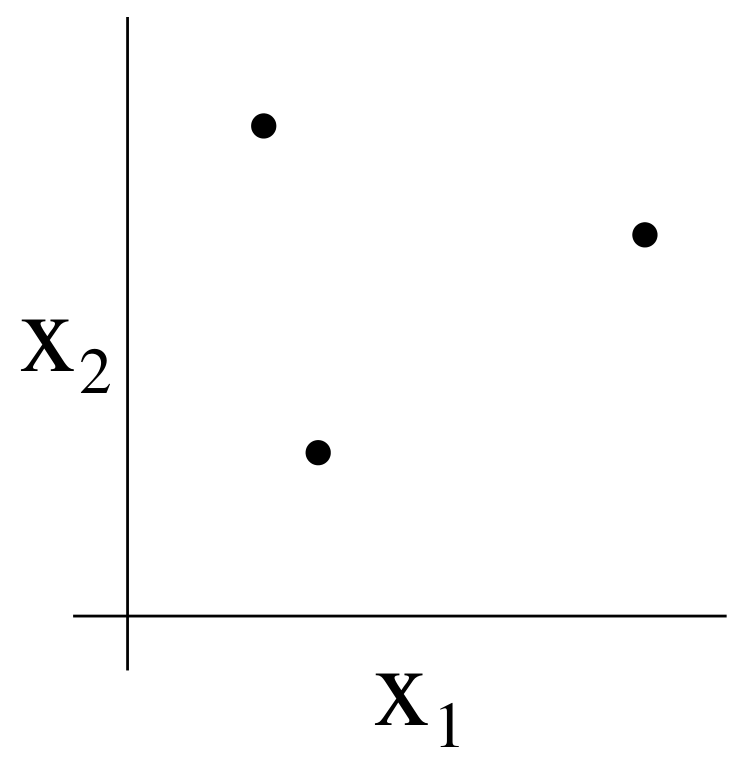
\includegraphics[width=0.4\linewidth]{figs/three_points.png}
\end{figure}

二维线性分类器组成的假设类 $\mathcal{H}$ ($h(x) = {1}\{\theta_0 + \theta_1 x_1 + \theta_2 x_2 \geq 0\}$) 能否打散上述集合?答案是肯定的。具体来说,我们看到,对于这八种可能的标记方式中的任何一种,我们都可以找到一个线性分类器,使得其在这三点上的“训练误差”为零:

\begin{figure}[H]
    \centering
    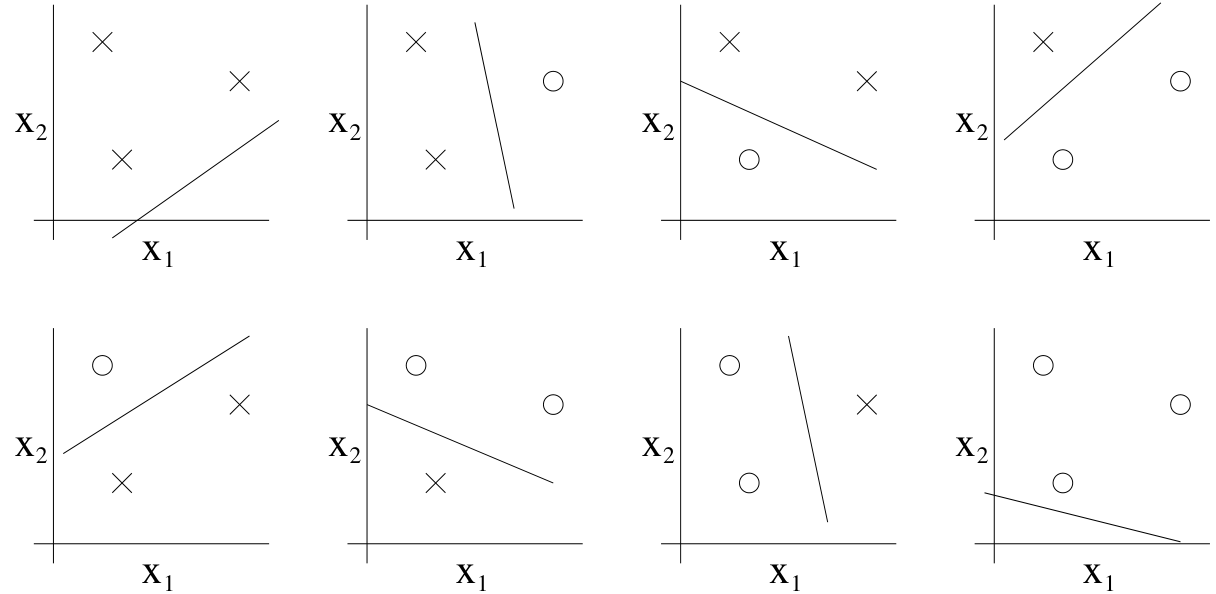
\includegraphics[width=0.9\linewidth]{figs/three_points_shatter.png}
\end{figure}

此外,可以证明不存在任何大小为 4 的点集是该假设类可以打散的。因此,$\mathcal{H}$ 可以打散的最大集合的大小为 3,所以 $\text{VC}(\mathcal{H}) = 3$。

注意,这里的 $\mathcal{H}$ 的 VC 维数为 3,即使可能存在一些大小为 3 的集合它无法打散。例如,如果我们有三个点共线(左图),那么对于下面右图所示的三个点的标记方式,无法找到一个线性分隔:

\begin{figure}[H]
    \centering
    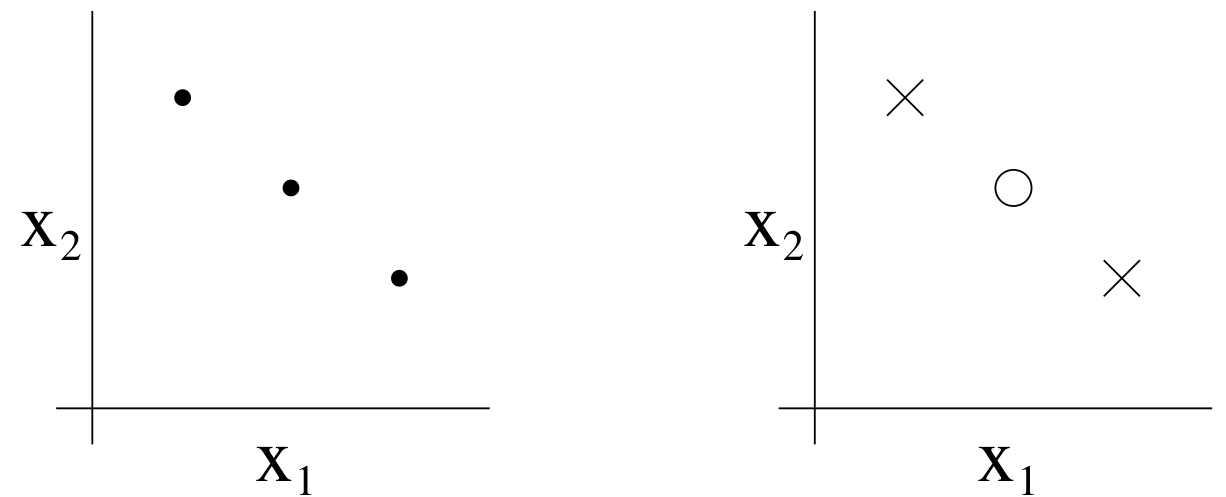
\includegraphics[width=0.9\linewidth]{figs/three_points_cant_shatter.png}
\end{figure}

换句话说,根据 VC 维数的定义,为了证明 $\text{VC}(\mathcal{H})$ 至少为 $\mathbf{D}$,我们只需要证明存在至少\textit{一个 (one)} 大小为 $\mathbf{D}$ 的集合是 $\mathcal{H}$ 可以打散的。

下面的定理由 Vapnik 证明。(许多人会认为这是学习理论中最重要的定理。)

\begin{theorem*}
    给定假设类 $\mathcal{H}$,令 $\mathbf{D} = \text{VC}(\mathcal{H})$。那么对于所有 $h \in \mathcal{H}$,以至少 $1-\delta$ 的概率有:
    \[
        |\varepsilon(h) - \hat{\varepsilon}(h)| \leq O\left(\sqrt{\frac{\mathbf{D}}{n} \log \frac{n}{\mathbf{D}} + \frac{1}{n} \log \frac{1}{\delta}}\right).
    \]
    因此,以至少 $1-\delta$ 的概率,也有:
    \[
        \varepsilon(\hat{h}) \leq \varepsilon(h^*) + O\left(\sqrt{\frac{\mathbf{D}}{n} \log \frac{n}{\mathbf{D}} + \frac{1}{n} \log \frac{1}{\delta}}\right).
    \]
\end{theorem*}

换句话说,如果一个假设类具有有限的 VC 维数,那么当 $n$ 变大时,就会产生一致收敛。像之前一样,这使得我们能够给出 $\varepsilon(\hat{h})$ 的一个界限,该界限以 $\varepsilon(h^*)$ 表示。我们还有下面的推论:

\begin{corollary*}
    对于所有 $h \in \mathcal{H}$,要使 $|\varepsilon(h) - \hat{\varepsilon}(h)| \leq \gamma$ 以至少 $1-\delta$ 的概率成立(因此 $\varepsilon(\hat{h}) \leq \varepsilon(h^*) + 2\gamma$),只需 $n = O_{\gamma, \delta}(\mathbf{D})$。
\end{corollary*}

换句话说,使 $\mathcal{H}$ 学习得“很好”,所需的训练样本数量与 $\mathcal{H}$ 的 VC 维数呈线性关系。结果表明,对于“大多数”假设类,VC 维数(假设“合理地”进行参数化)也与参数数量大致呈线性关系。将这些结合起来,我们得出结论:对于给定的假设类 $\mathcal{H}$(以及最小化训练误差的算法),达到接近最优分类器泛化误差所需的训练样本数量通常与 $\mathcal{H}$ 的参数数量大致呈线性关系。